%!TEX root = ../main.tex
\section{Task-driven Data Preparation}
\label{sec:dataprep}



In the era of big data, from the data perspective, the data can come from governments, business companies, Web, and so on. 
As shown in Figure~\ref{fig:framwork}, in the scenario of COVID-19, the data can come from WHO, each country's Center for Disease Control and Prevention (CDC), news websites, microblog text,  and other statistic datasets (\eg population, temperature and international airline data). 
In addition to heterogeneous data sources, how to integrate data with different data formats (\eg table, JSON-like, and text) from different data sources is another problem.
One concrete example is how to extract the data from the CDC daily reports and then align such data into predefined relational tables.
In this work, we develop an algorithm to crawl, extract data and fill them into relational tables.

%After collecting and integrating data, the next problem is to detect and repair data errors.
Clean data is one of the essential requirements for data analytics and accurate analysis results~\cite{DBLP:journals/pvldb/AbedjanCDFIOPST16, DBLP:conf/cidr/BinnigSKUZZ17}. However, data collection and integration usually introduce errors (\eg missing values, mixed formats, and duplicates) in data due to the integration of heterogeneous data sources~\cite{10.14778/3137765.3137833}. 
%
As shown in the Figure~\ref{fig:data_errors}(a), they are four types of common data errors in the scenario of COVID-19. 
%
First, the synonyms usually appear when integrating data from different sources, especially when the data standard of data sources may change. 
%
The second data errors is missing value, as shown in Figure~\ref{fig:data_errors}(b), this type of data error is usually caused by the data source not being updated in time. 
More concretely, on the 05/02, the data source may not have published the total number of deaths on that day, so a missing value was introduced. The missing value imputation is usually estimated using the data of the first few days and later, or imputation by querying other data sources.
%
Similar to the missing value, as shown in Figure~\ref{fig:data_errors}(c), it may also introduce incorrect values. We use the average values of the data of the first few days and later as a repair candidate to correct the wrong value.
%
As shown in Figure~\ref{fig:data_errors}(d), we crawl the travel records of some infected people from the news website. However, because data is crawled from multiple websites and then integrated, it is easy to introduce duplicate records. For duplicate records, we can use the entity matching algorithm to detect and remove duplicate records.
%

Because the analysis scenarios of COVID-19 have high requirements on data quality, we first need to ensure the data quality, and then consider how to reduce the cost of data cleaning.
However, it's too expensive and infeasible to resolve all errors.
Therefore, we discuss how to conduct problem-oriented (task-driven) data cleaning for COVID-19. 
The key idea is that we only clean those data relevant to the data analytics tasks, which can reduce the cost of data cleaning.
In other words, instead of applying cleaning tools to clean each type of data errors before visualization, we aim to clean those data errors that have heavy impact on the accuracy of the visualization results.
We devise our recent technique, a framework for visualization-aware data cleaning, called \textsc{VisClean} to achieve this goal.
The key idea is that we first generate visualizations based on the possible dirty dataset, and then run cleaning tools in the backend to find possible errors and their repairing candidates. Next, we organize those data errors and their repairing candidates by a graph model. Based on the graph and a predefined benefit model, we aim to select the most ``beneficial'' questions to interact with the user. The large the benefit is, the high quality of visualization improvement is. After the user answer the data cleaning questions, the system will fix data errors and refresh the visualization.
%
%\add{We may first give a general idea and a sketch of our solution. We can then give one concrete example using COVID-19 data. One example might be joining two tables, for population or for continent info, but you found out that the names are not normalized. Instead of normalizing all names, you can only normalize the data that is relevant for your task, 
%eg when comparing hong kong, tai wai, etc, the names are not normalized.}

%%%%%%%%%%%%%%%%%%%%%%%%%%%%%%%%%%%%
\begin{figure}[t!]
	\centering
	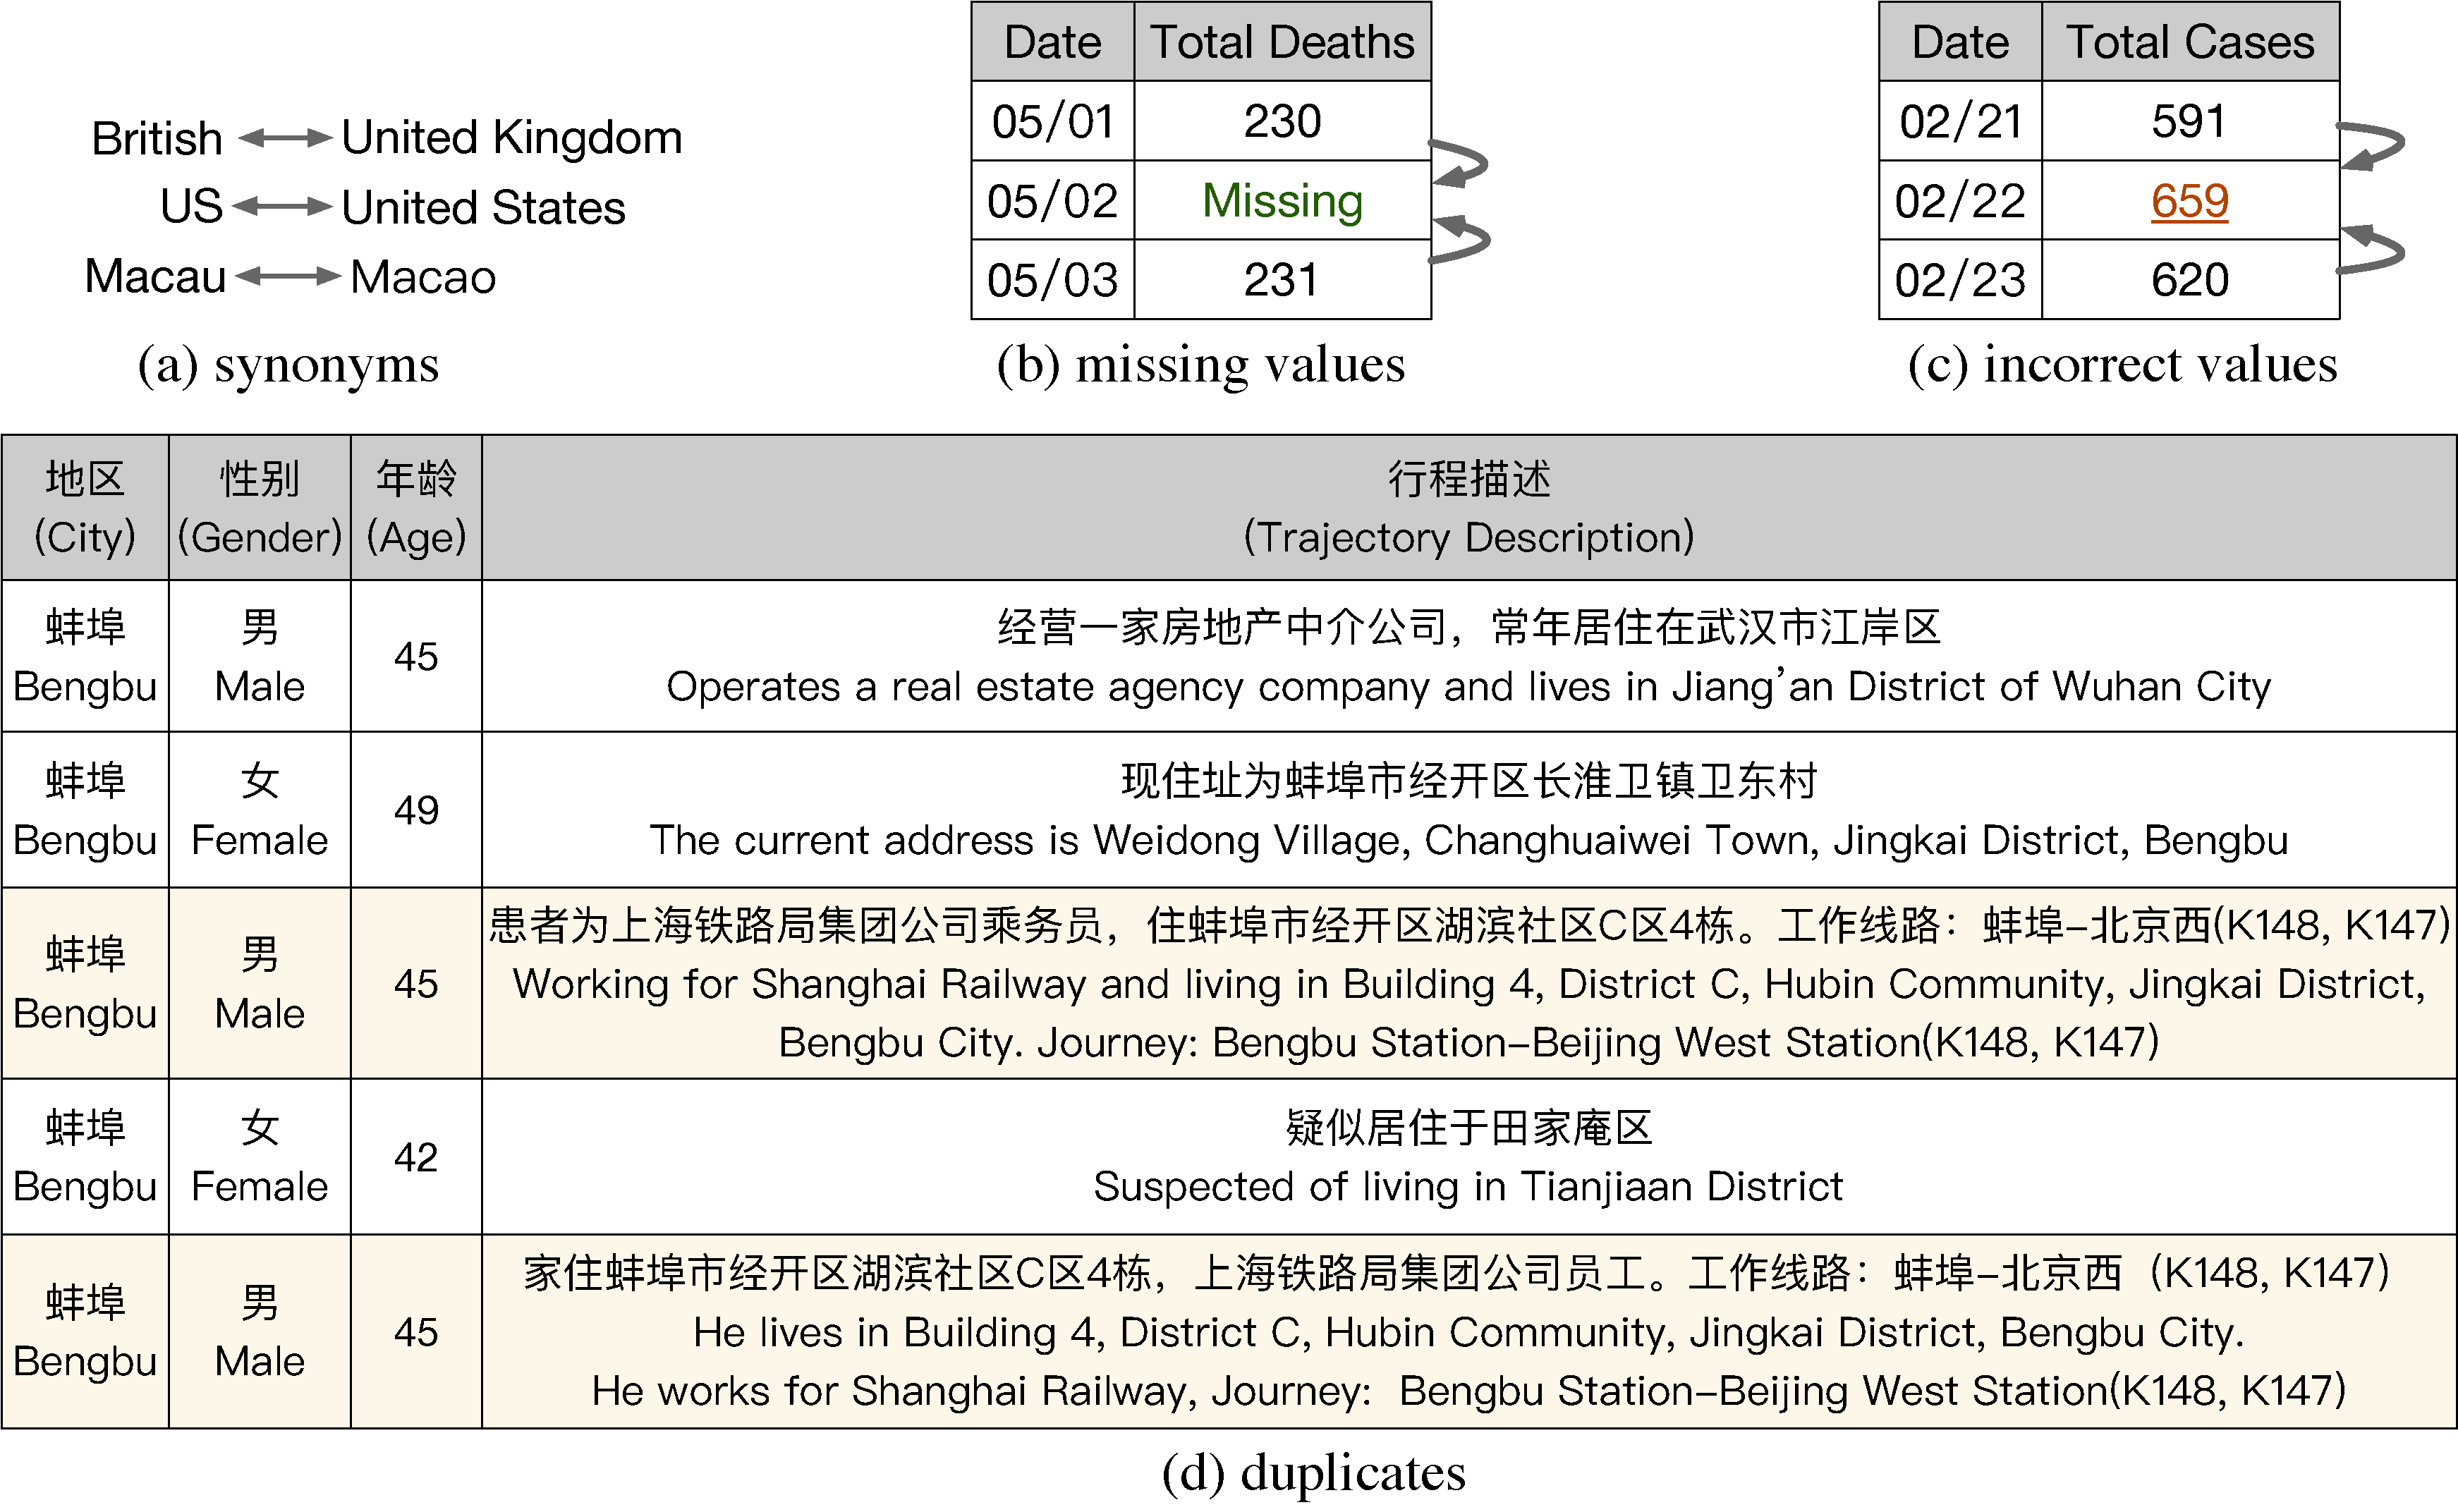
\includegraphics[width=.85\columnwidth]{figs/data_errors.pdf}
	\vspace{-1em}
	\caption{Examples of Data Errors}
	\label{fig:data_errors}
	\vspace{-1em}
\end{figure}
%%%%%%%%%%%%%%%%%%%%%%%%%%%%%%%%%%%

%\add{The idea of VisClean is not given here. What you describe above are the types of errors. We should definitely describe the idea of VisClean or better shows how it works by using the errors in Figure 3.}